\section{Rectificador}
La rectificación es el proceso de convertir una forma de onda de corriente
alterna en una forma de onda de corriente continua (en este caso, variable) que
tiene una sola polaridad.

\subsection{Media onda}
Considerando el circuito de la \textbf{figura~\ref{circuito02}}, se aprecia un
bucle en serie que consiste en una fuente de onda sinusoidal conectada a un
transformador; desde el transformador se conecta un diodo \textbf{1N4007} y una
resistencia de $10[\text{k}\Omega]$ que cumple la funcion de carga.

\begin{figure}[!h]
\centering
\includegraphics[scale=1]{diagramas/02.media_onda1.eps}
\caption{Rectificador de media onda.}
\label{circuito02}
\end{figure}

Para los valores positivos del voltaje de entrada, el diodo estará polarizado
directamente, por tanto la señal de entrada caerá a través de la resistencia de
carga; mientras que con los valores negativos del voltaje de entrada, hará que
el diodo este polarizado inversamente y por tanto no circulará corriente a
traves de la carga.

\subsubsection{Simulación}
Se utilizó el software \emph{Quite Universal Circuit Simulator.} versión 23.3.1
para la simulación del rectificador de media onda, este puede verse en la
\textbf{figura~\ref{simulacion02}}.

\begin{figure}[!h]
\centering
\includegraphics[scale=0.75]{simulacion/02.media_onda1.eps}
\caption{Simulación del rectificador de media onda.}
\label{simulacion02}
\end{figure}

\subsubsection{Laboratorio}
Se presenta el rectificador de media onda armado en laboratorio y su medición
de voltaje de salida en la carga, en la \textbf{figura~\ref{laboratorio04}}.

\begin{figure}[!h]
\centering
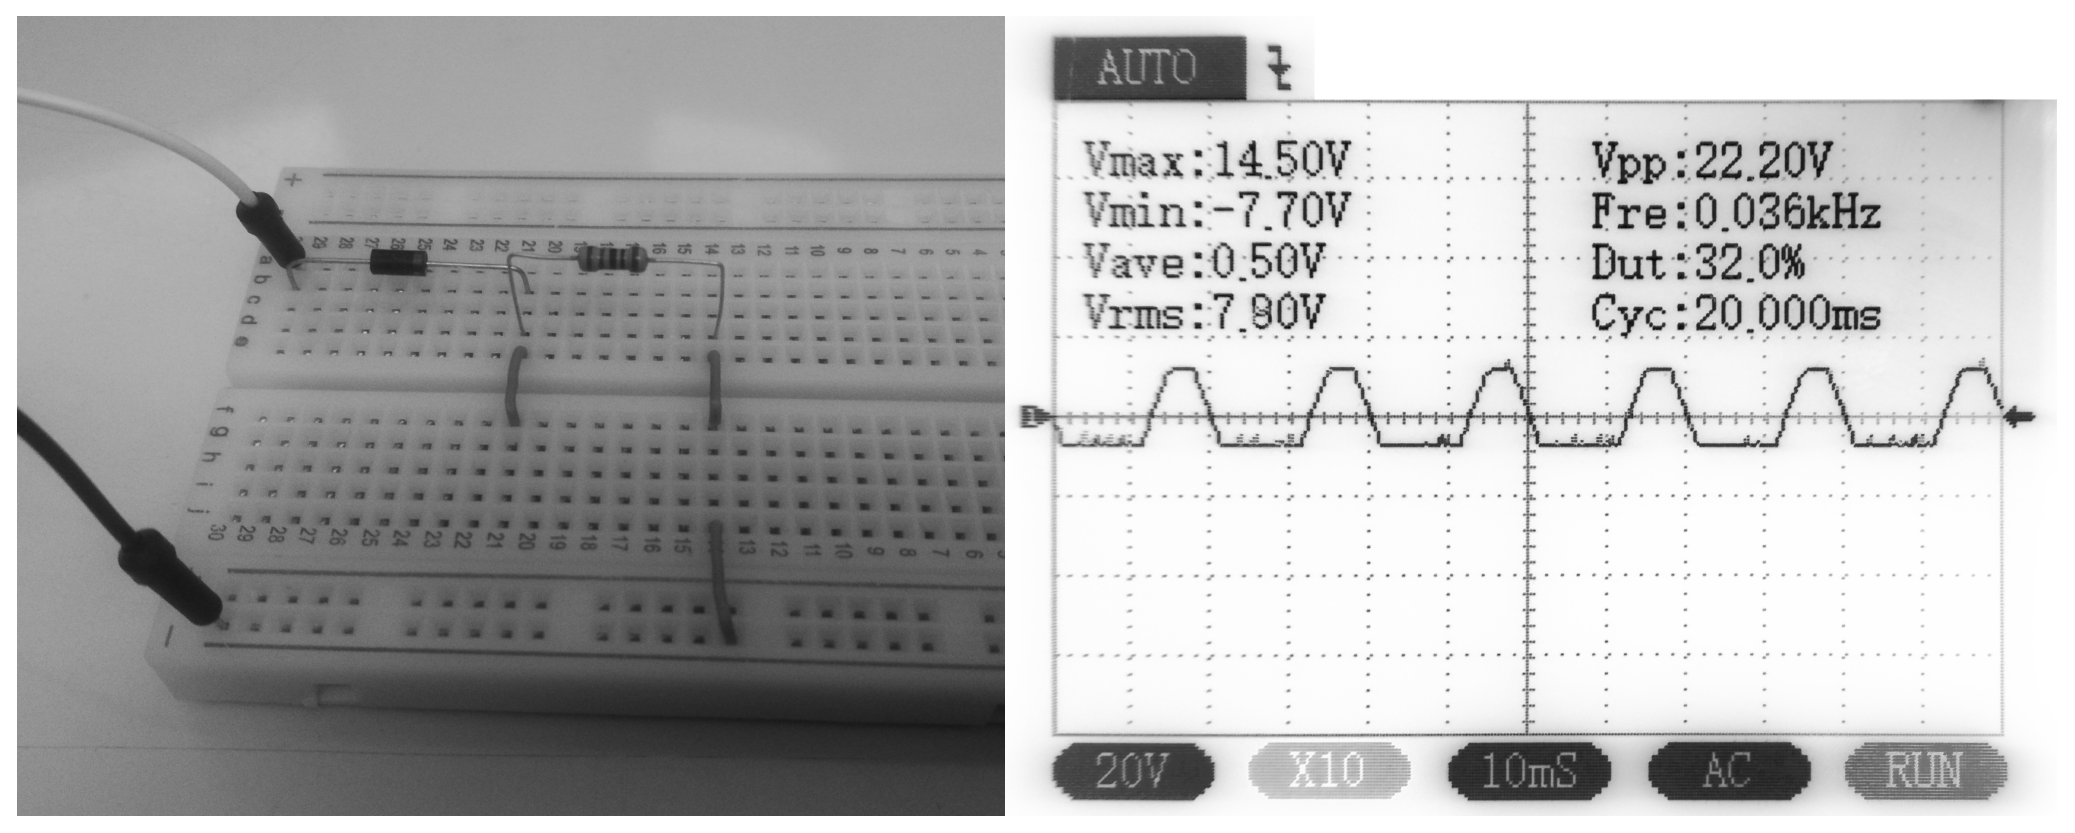
\includegraphics[scale=0.28]{fotos/02.media_onda1.eps}
\caption{Rectificador de media onda.}
\label{laboratorio04}
\end{figure}

\subsection{Onda completa con derivación central}
Este rectificador utiliza dos diodos \textbf{1N4007} conectados a un
transformador con derivación central y una resistencia de $10[\text{k}\Omega]$
que cumple la funcion de carga, como se muestra en la
\textbf{figura~\ref{circuito03}}, los voltajes entre las terminales del
transformador son iguales en magnitud, pero con diferentes fases.

\begin{figure}[!h]
\centering
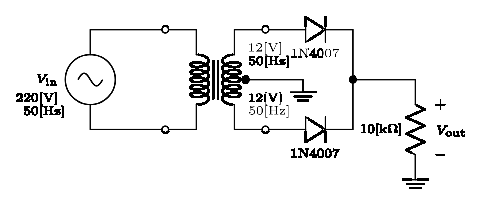
\includegraphics[scale=1]{diagramas/03.derivacion_central1.eps}
\caption{Rectificador de onda completa con transformador de derivación central.}
\label{circuito03}
\end{figure}

La polarización directa e inversa son alternadas en cada diodo del circuito por
lo que se obtienen solo los valores positivos de cada extremo del transformador.

\subsubsection{Simulación}
Se utilizó el software \emph{Quite Universal Circuit Simulator.} versión 23.3.1
para la simulación del rectificador de onda completa, este puede verse en la
\textbf{figura~\ref{simulacion03}}.

\begin{figure}[!h]
\centering
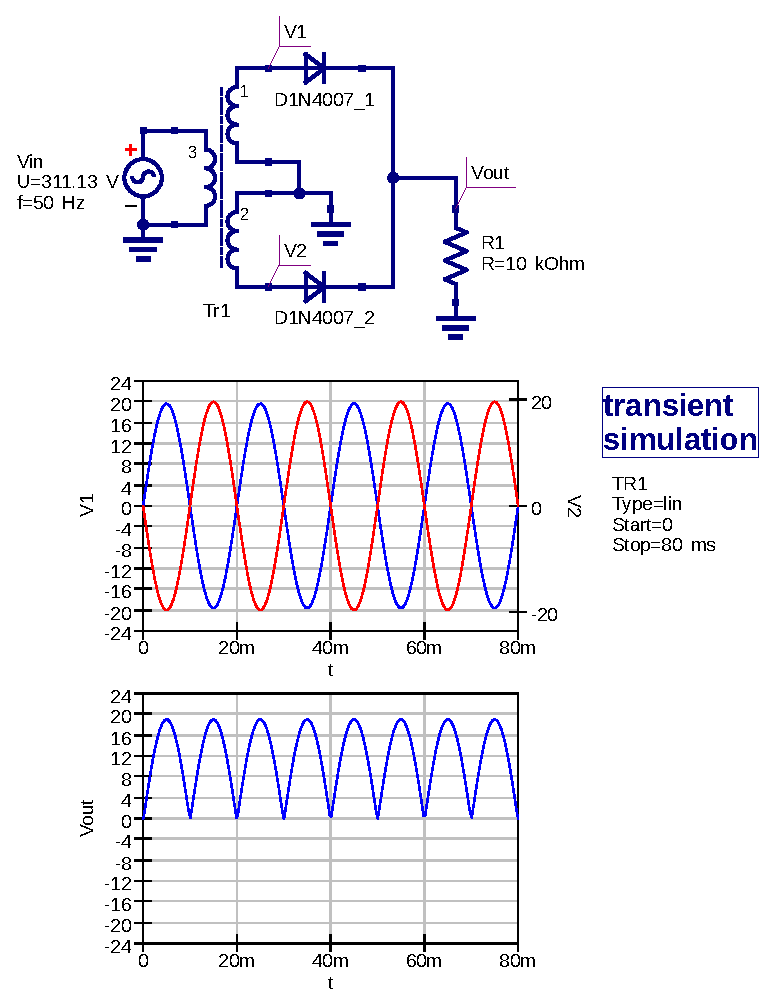
\includegraphics[scale=0.75]{simulacion/03.derivacion_central1.eps}
\caption{Simulación del rectificador de onda completa con derivacion central.}
\label{simulacion03}
\end{figure}

\subsubsection{Laboratorio}
Se presenta el rectificador de onda completa con el transformador de derivación
central armado en laboratorio y su medición de voltaje de salida en la carga, en
la \textbf{figura~\ref{laboratorio05}}.

\begin{figure}[!h]
\centering
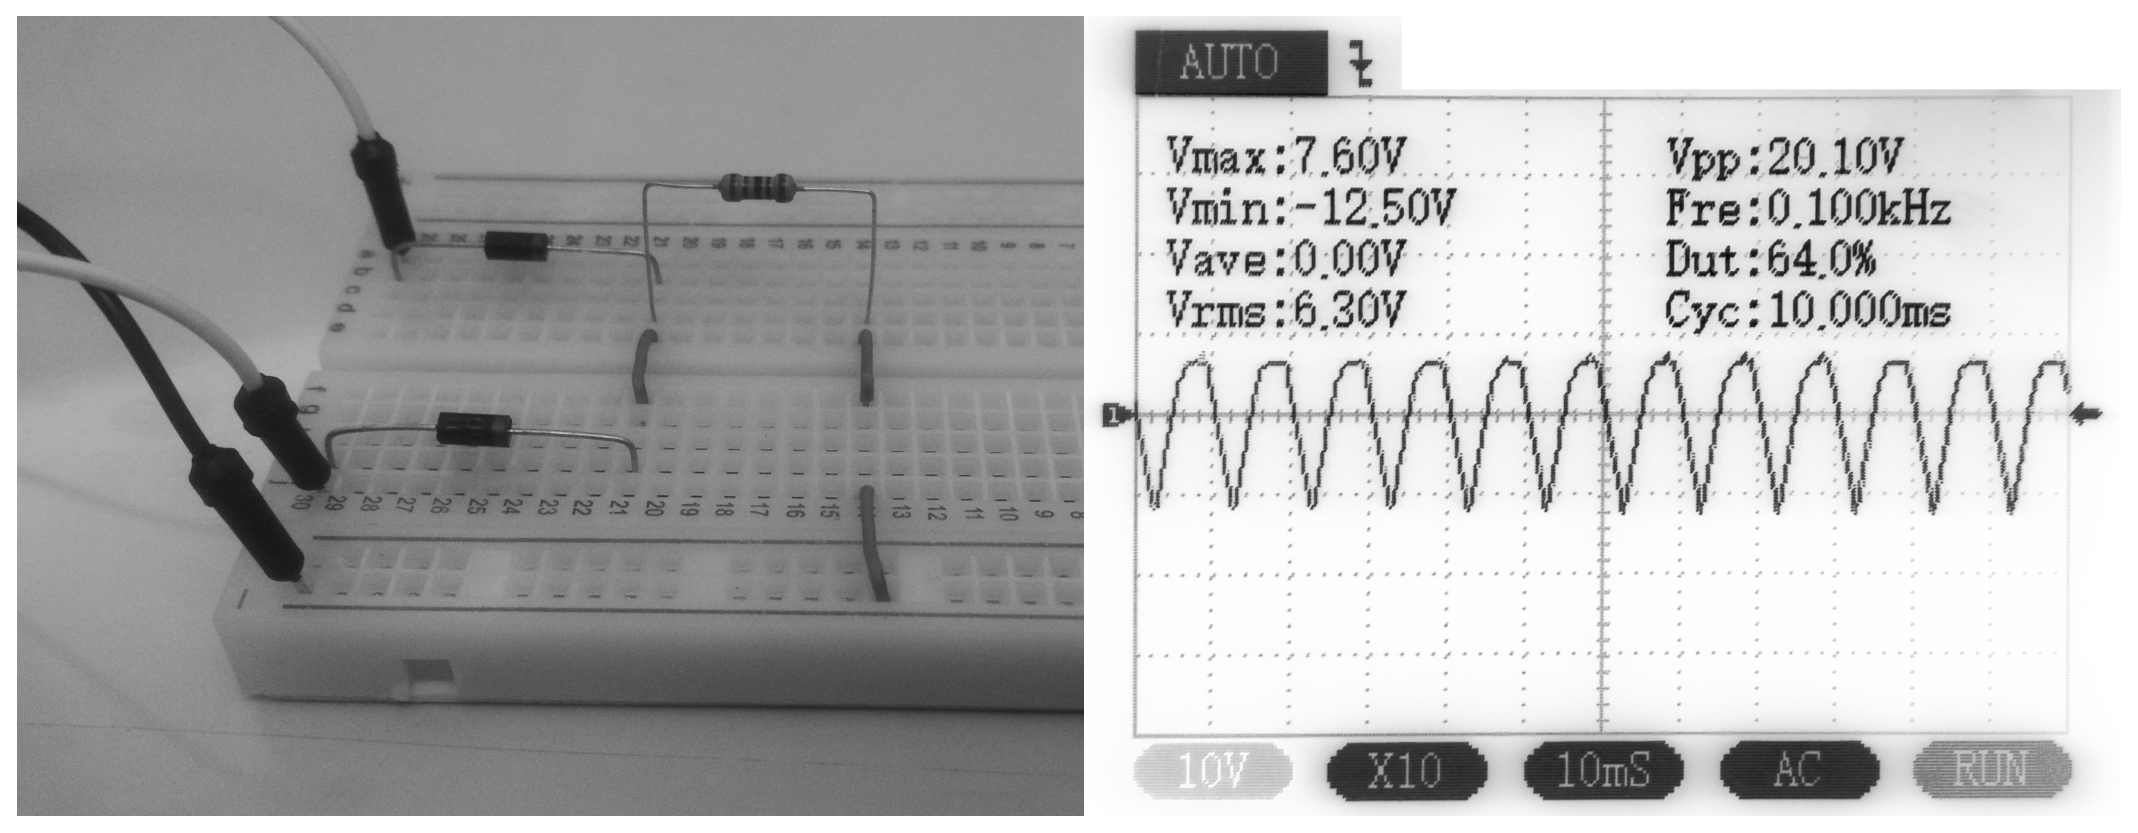
\includegraphics[scale=0.28]{fotos/03.derivacion_central1.eps}
\caption{Rectificador de onda completa con derivación central.}
\label{laboratorio05}
\end{figure}

\subsection{Onda completa de puente}
Este rectificador utiliza cuatro diodos \textbf{1N4007} conectados como un
puente y conectados a una resistencia de $10[\text{k}\Omega]$, como se muestra
en la \textbf{figura~\ref{circuito04}}.

\begin{figure}[!h]
\centering
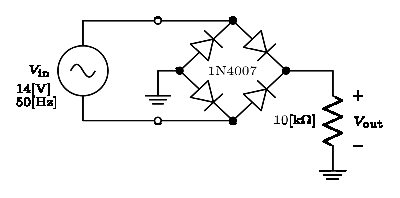
\includegraphics[scale=1]{diagramas/04.onda_completa1.eps}
\caption{Rectificador de onda completa con puente.}
\label{circuito04}
\end{figure}

Los valores positivos del voltaje de entrada polariza directamente a dos diodos
y polariza inversamente a los dos diodos restantes, mientras que los valores
negativos del voltaje hace el camino contrario por los diodos del circuito, lo
que genera la señal de onda completa con el doble de la frecuencia del voltaje
de entrada.

\subsubsection{Simulación}
Se utilizó el software \emph{Quite Universal Circuit Simulator.} versión 23.3.1
para la simulación del rectificador de onda completa, este puede verse en la
\textbf{figura~\ref{simulacion04}}.

\begin{figure}[!h]
\centering
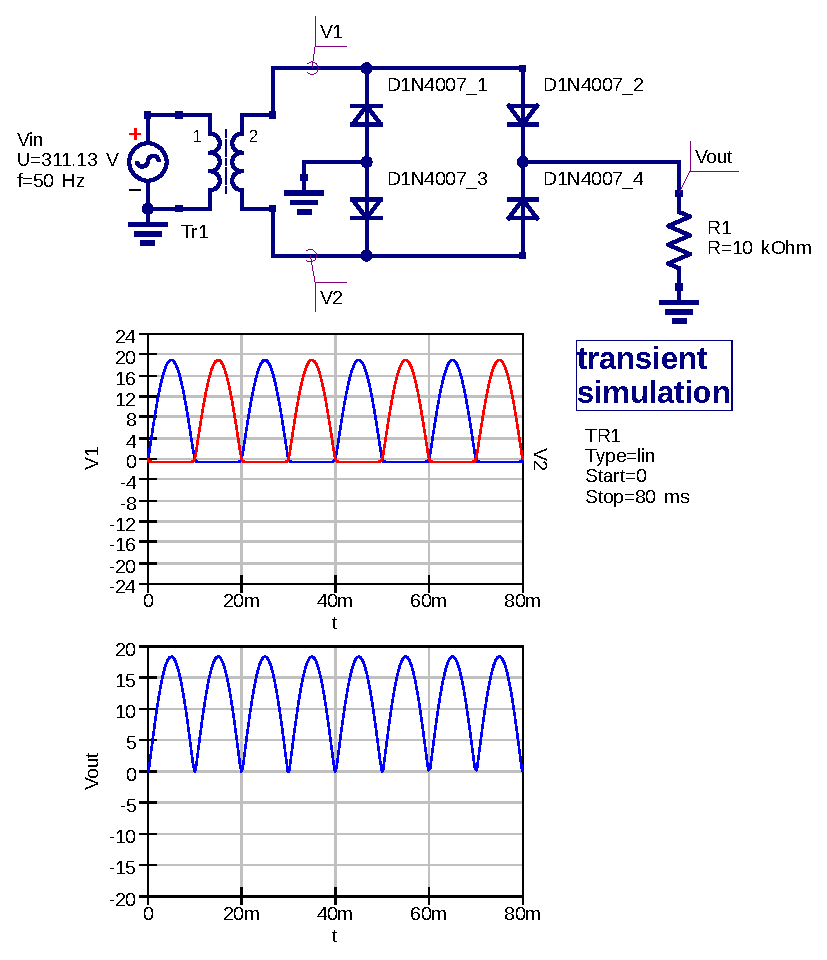
\includegraphics[scale=0.75]{simulacion/04.onda_completa1.eps}
\caption{Simulación del rectificador de onda completa con puente.}
\label{simulacion04}
\end{figure}

\subsubsection{Laboratorio}
Se presenta el rectificador de onda completa con puente armado en laboratorio y
su medición de voltaje de salida en la carga, en la
\textbf{figura~\ref{laboratorio06}}.

\begin{figure}[!h]
\centering
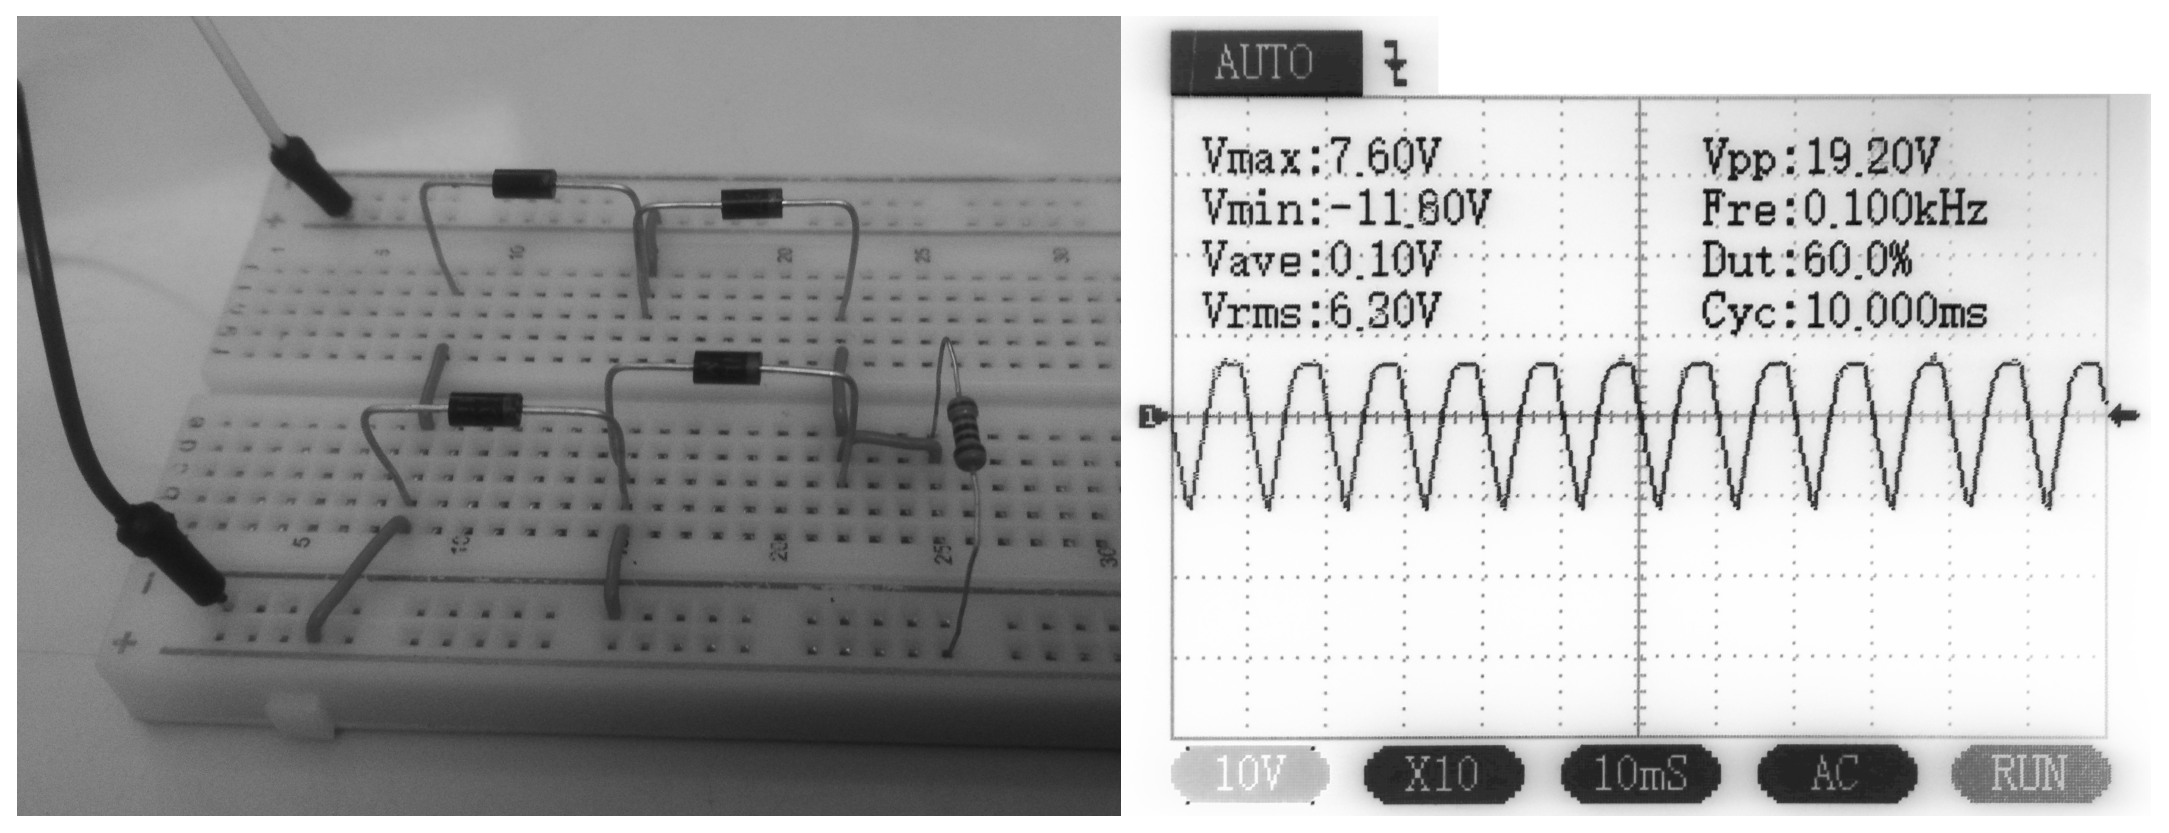
\includegraphics[scale=0.28]{fotos/04.onda_completa1.eps}
\caption{Rectificador de onda completa con puente.}
\label{laboratorio06}
\end{figure}

